% Options for packages loaded elsewhere
\PassOptionsToPackage{unicode}{hyperref}
\PassOptionsToPackage{hyphens}{url}
%
\documentclass[
]{book}
\title{Estadística Aplicada a las Ciencias y la Ingeniería}
\author{Emilio L. Cano}
\date{2021-08-31}

\usepackage{amsmath,amssymb}
\usepackage{lmodern}
\usepackage{iftex}
\ifPDFTeX
  \usepackage[T1]{fontenc}
  \usepackage[utf8]{inputenc}
  \usepackage{textcomp} % provide euro and other symbols
\else % if luatex or xetex
  \usepackage{unicode-math}
  \defaultfontfeatures{Scale=MatchLowercase}
  \defaultfontfeatures[\rmfamily]{Ligatures=TeX,Scale=1}
\fi
% Use upquote if available, for straight quotes in verbatim environments
\IfFileExists{upquote.sty}{\usepackage{upquote}}{}
\IfFileExists{microtype.sty}{% use microtype if available
  \usepackage[]{microtype}
  \UseMicrotypeSet[protrusion]{basicmath} % disable protrusion for tt fonts
}{}
\makeatletter
\@ifundefined{KOMAClassName}{% if non-KOMA class
  \IfFileExists{parskip.sty}{%
    \usepackage{parskip}
  }{% else
    \setlength{\parindent}{0pt}
    \setlength{\parskip}{6pt plus 2pt minus 1pt}}
}{% if KOMA class
  \KOMAoptions{parskip=half}}
\makeatother
\usepackage{xcolor}
\IfFileExists{xurl.sty}{\usepackage{xurl}}{} % add URL line breaks if available
\IfFileExists{bookmark.sty}{\usepackage{bookmark}}{\usepackage{hyperref}}
\hypersetup{
  pdftitle={Estadística Aplicada a las Ciencias y la Ingeniería},
  pdfauthor={Emilio L. Cano},
  hidelinks,
  pdfcreator={LaTeX via pandoc}}
\urlstyle{same} % disable monospaced font for URLs
\usepackage{color}
\usepackage{fancyvrb}
\newcommand{\VerbBar}{|}
\newcommand{\VERB}{\Verb[commandchars=\\\{\}]}
\DefineVerbatimEnvironment{Highlighting}{Verbatim}{commandchars=\\\{\}}
% Add ',fontsize=\small' for more characters per line
\usepackage{framed}
\definecolor{shadecolor}{RGB}{248,248,248}
\newenvironment{Shaded}{\begin{snugshade}}{\end{snugshade}}
\newcommand{\AlertTok}[1]{\textcolor[rgb]{0.94,0.16,0.16}{#1}}
\newcommand{\AnnotationTok}[1]{\textcolor[rgb]{0.56,0.35,0.01}{\textbf{\textit{#1}}}}
\newcommand{\AttributeTok}[1]{\textcolor[rgb]{0.77,0.63,0.00}{#1}}
\newcommand{\BaseNTok}[1]{\textcolor[rgb]{0.00,0.00,0.81}{#1}}
\newcommand{\BuiltInTok}[1]{#1}
\newcommand{\CharTok}[1]{\textcolor[rgb]{0.31,0.60,0.02}{#1}}
\newcommand{\CommentTok}[1]{\textcolor[rgb]{0.56,0.35,0.01}{\textit{#1}}}
\newcommand{\CommentVarTok}[1]{\textcolor[rgb]{0.56,0.35,0.01}{\textbf{\textit{#1}}}}
\newcommand{\ConstantTok}[1]{\textcolor[rgb]{0.00,0.00,0.00}{#1}}
\newcommand{\ControlFlowTok}[1]{\textcolor[rgb]{0.13,0.29,0.53}{\textbf{#1}}}
\newcommand{\DataTypeTok}[1]{\textcolor[rgb]{0.13,0.29,0.53}{#1}}
\newcommand{\DecValTok}[1]{\textcolor[rgb]{0.00,0.00,0.81}{#1}}
\newcommand{\DocumentationTok}[1]{\textcolor[rgb]{0.56,0.35,0.01}{\textbf{\textit{#1}}}}
\newcommand{\ErrorTok}[1]{\textcolor[rgb]{0.64,0.00,0.00}{\textbf{#1}}}
\newcommand{\ExtensionTok}[1]{#1}
\newcommand{\FloatTok}[1]{\textcolor[rgb]{0.00,0.00,0.81}{#1}}
\newcommand{\FunctionTok}[1]{\textcolor[rgb]{0.00,0.00,0.00}{#1}}
\newcommand{\ImportTok}[1]{#1}
\newcommand{\InformationTok}[1]{\textcolor[rgb]{0.56,0.35,0.01}{\textbf{\textit{#1}}}}
\newcommand{\KeywordTok}[1]{\textcolor[rgb]{0.13,0.29,0.53}{\textbf{#1}}}
\newcommand{\NormalTok}[1]{#1}
\newcommand{\OperatorTok}[1]{\textcolor[rgb]{0.81,0.36,0.00}{\textbf{#1}}}
\newcommand{\OtherTok}[1]{\textcolor[rgb]{0.56,0.35,0.01}{#1}}
\newcommand{\PreprocessorTok}[1]{\textcolor[rgb]{0.56,0.35,0.01}{\textit{#1}}}
\newcommand{\RegionMarkerTok}[1]{#1}
\newcommand{\SpecialCharTok}[1]{\textcolor[rgb]{0.00,0.00,0.00}{#1}}
\newcommand{\SpecialStringTok}[1]{\textcolor[rgb]{0.31,0.60,0.02}{#1}}
\newcommand{\StringTok}[1]{\textcolor[rgb]{0.31,0.60,0.02}{#1}}
\newcommand{\VariableTok}[1]{\textcolor[rgb]{0.00,0.00,0.00}{#1}}
\newcommand{\VerbatimStringTok}[1]{\textcolor[rgb]{0.31,0.60,0.02}{#1}}
\newcommand{\WarningTok}[1]{\textcolor[rgb]{0.56,0.35,0.01}{\textbf{\textit{#1}}}}
\usepackage{longtable,booktabs,array}
\usepackage{calc} % for calculating minipage widths
% Correct order of tables after \paragraph or \subparagraph
\usepackage{etoolbox}
\makeatletter
\patchcmd\longtable{\par}{\if@noskipsec\mbox{}\fi\par}{}{}
\makeatother
% Allow footnotes in longtable head/foot
\IfFileExists{footnotehyper.sty}{\usepackage{footnotehyper}}{\usepackage{footnote}}
\makesavenoteenv{longtable}
\usepackage{graphicx}
\makeatletter
\def\maxwidth{\ifdim\Gin@nat@width>\linewidth\linewidth\else\Gin@nat@width\fi}
\def\maxheight{\ifdim\Gin@nat@height>\textheight\textheight\else\Gin@nat@height\fi}
\makeatother
% Scale images if necessary, so that they will not overflow the page
% margins by default, and it is still possible to overwrite the defaults
% using explicit options in \includegraphics[width, height, ...]{}
\setkeys{Gin}{width=\maxwidth,height=\maxheight,keepaspectratio}
% Set default figure placement to htbp
\makeatletter
\def\fps@figure{htbp}
\makeatother
\setlength{\emergencystretch}{3em} % prevent overfull lines
\providecommand{\tightlist}{%
  \setlength{\itemsep}{0pt}\setlength{\parskip}{0pt}}
\setcounter{secnumdepth}{5}
\usepackage{booktabs}
\usepackage[spanish, es-tabla]{babel}

\usepackage{framed,color}
\definecolor{shadecolor}{RGB}{248,248,248}

\newenvironment{rmdejemplo}
  {\begin{rmdblock}{ejemplo}}
  {\end{rmdblock}}
\newenvironment{rmdcafe}
  {\begin{rmdblock}{cafe}}
  {\end{rmdblock}}
\newenvironment{rmdpractica}
  {\begin{rmdblock}{practice}}
  {\end{rmdblock}}
\newenvironment{rmdpremium}
  {\begin{rmdblock}{premium}}
  {\end{rmdblock}}
  
\ifLuaTeX
  \usepackage{selnolig}  % disable illegal ligatures
\fi
\usepackage[]{natbib}
\bibliographystyle{apalike}

\begin{document}
\maketitle

{
\setcounter{tocdepth}{1}
\tableofcontents
}
\hypertarget{prefacio}{%
\chapter*{Prefacio}\label{prefacio}}
\addcontentsline{toc}{chapter}{Prefacio}

Este libro incluye los contenidos habitualmente presentes en el currículo
de asignaturas de \textbf{Estadística} de los grados Ciencias e Ingenierías de universidades españolas.
Si bien existe abundante material bibliográfico
que cubre los contenidos de estas asignaturas, quería elaborar un material
propio que no fuera solamente para mis clases sino algo más
\emph{global}. Por otra parte, me motiva cubrir el hueco de los materiales
de acceso gratuito con la opción de comprar una edición
impresa\footnote{A la espera de encontrar editorial.} y con el enfoque
que se menciona en el siguiente apartado. Por otra parte, los libros publicados
originalmente en inglés y traducidos al español a menudo me resultan lejanos
a nuestro idioma (por muy buenas que sean las traducciones, los ejemplos en \emph{acres}
no son muy intuitivos para un lector español). Espero que también sirva para
lectores de otros países de habla hispana.

\hypertarget{estuxe1ndares-y-software}{%
\section*{Estándares y software}\label{estuxe1ndares-y-software}}
\addcontentsline{toc}{section}{Estándares y software}

Los contenidos de este libro se basan en dos paradigmas que están presentes
en los intereses de investigación y docencia del autor: los \textbf{estándares} y
el \textbf{software libre}. En lo que se refiere a estándares, la notación utilizada,
definiciones y fórmulas se ajustarán el máximo posible a la utilizada en normas
nacionales e internacionales sobre metodología estadística. Estas normas se
citarán pertinentemente a lo largo del texto. En cuanto al software libre,
se proporcionarán instrucciones para resolver los ejemplos
que ilustran la teoría utilizando software libre.
No obstante, el uso del software es
auxiliar al texto y se puede seguir sin necesidad de utilizar
los programas. Según lo que proceda en cada caso, se utilizará
software de hoja de cálculo, el software estadístico y lenguaje de
programación
\textbf{R} \citep{R-base},
y el software de álgebra computacional \textbf{Máxima}\footnote{\url{http://maxima.sourceforge.net/es/}}.
Respecto al software de hoja de cálculo, las fórmulas utilizadas se han probado
en el software libre \textbf{LibreOffice}\footnote{\url{https://es.libreoffice.org}}, en \textbf{Hojas de Cálculo de Google}\footnote{\url{https://www.google.es/intl/es/sheets/about/}} y
también en \textbf{Microsoft EXCEL}\footnote{\url{https://products.office.com/es-es/excel}} que,
aunque no es software libre, su uso
está más que generalizado y normalmente los estudiantes disponen de licencia de uso
a través de su universidad. En caso de que el nombre de la función sea distinta
en EXCEL, se indicará en el propio ejemplo.

Las normas son clave para el desarrollo económico de un país. Estudios en diversos países,
incluido España, han demostrado que la aportación de la normalización a su economía es del 1\% del PIB\footnote{\url{http://www.aenor.es/DescargasWeb/normas/como-beneficia-es.pdf}}. La
Asociación Española de Normalización (UNE) es el organismo legalmente
responsable del desarrollo y difusión de las normas técnicas en España.
Además, representa a España en los organismos internacionales de normalización como
\href{https://www.iso.org/}{ISO}\footnote{\url{https://www.iso.org/}} y \href{https://www.cen.eu/}{CEN}\footnote{\url{https://www.cen.eu/}}.

Las normas sobre estadística que surgen de ISO las elabora el \emph{Technical Committee}
ISO TC 69\footnote{\url{https://www.iso.org/committee/49742/x/catalogue/}} \emph{Statistical Methods}.
Por su parte, el subcomité técnico de normalización
CTN 66/SC 3\footnote{\url{https://www.une.org/encuentra-tu-norma/comites-tecnicos-de-normalizacion/comite/?c=CTN\%2066/SC\%203}}, Métodos Estadísticos,
participa como miembro nacional en ese comité ISO.
Las normas que son de interés en España, se ratifican en inglés o se traducen
al español como normas UNE. Para una descripción más completa de la elaboración
de normas, véase \citet{cano2015qcr}.

Este libro se ha elaborado utilizando el lenguaje \emph{Markdown} con el propio
software \textbf{R} y el paquete \textbf{bookdown} \citep{R-bookdown}.
Se incluyen una gran cantidad de ejemplos resueltos tanto de forma analítica
como mediante software. En algunos casos se proporciona el uso de funciones
en hojas de cálculo (y el resultado obtenido con un recuadro).
En otros, código de R, que aparecen en el texto
sombreados y con la sintaxis coloreada, como el fragmento a continuación
donde se puede comprobar la sesión de R en la que ha sido generado este material.
Obsérvese que los resultados se muestran precedidos de los símbolos
\texttt{\#\textgreater{}}.

\begin{Shaded}
\begin{Highlighting}[]
\FunctionTok{sessionInfo}\NormalTok{()}
\CommentTok{\#\textgreater{} R version 4.1.1 (2021{-}08{-}10)}
\CommentTok{\#\textgreater{} Platform: x86\_64{-}apple{-}darwin17.0 (64{-}bit)}
\CommentTok{\#\textgreater{} Running under: macOS Big Sur 10.16}
\CommentTok{\#\textgreater{} }
\CommentTok{\#\textgreater{} Matrix products: default}
\CommentTok{\#\textgreater{} BLAS:   /Library/Frameworks/R.framework/Versions/4.1/Resources/lib/libRblas.0.dylib}
\CommentTok{\#\textgreater{} LAPACK: /Library/Frameworks/R.framework/Versions/4.1/Resources/lib/libRlapack.dylib}
\CommentTok{\#\textgreater{} }
\CommentTok{\#\textgreater{} locale:}
\CommentTok{\#\textgreater{} [1] es\_ES.UTF{-}8/es\_ES.UTF{-}8/es\_ES.UTF{-}8/C/es\_ES.UTF{-}8/es\_ES.UTF{-}8}
\CommentTok{\#\textgreater{} }
\CommentTok{\#\textgreater{} attached base packages:}
\CommentTok{\#\textgreater{} [1] stats     graphics  grDevices utils     datasets }
\CommentTok{\#\textgreater{} [6] methods   base     }
\CommentTok{\#\textgreater{} }
\CommentTok{\#\textgreater{} loaded via a namespace (and not attached):}
\CommentTok{\#\textgreater{}  [1] compiler\_4.1.1  magrittr\_2.0.1  fastmap\_1.1.0  }
\CommentTok{\#\textgreater{}  [4] bookdown\_0.23.4 htmltools\_0.5.2 tools\_4.1.1    }
\CommentTok{\#\textgreater{}  [7] yaml\_2.2.1      stringi\_1.7.4   rmarkdown\_2.10 }
\CommentTok{\#\textgreater{} [10] knitr\_1.33      stringr\_1.4.0   digest\_0.6.27  }
\CommentTok{\#\textgreater{} [13] xfun\_0.25       rlang\_0.4.11    evaluate\_0.14}
\end{Highlighting}
\end{Shaded}

Normalmente, la descripción o enunciado de los ejemplos se incluyen en bloques
con el siguiente aspecto:

Esto es un ejemplo. A continuación puede mostrarse código o no.

Cuando el ejemplo incluya explicaciones sobre cómo resolverlo con software,
estas explicaciones aparecerán en bloques con el siguiente aspecto:

\textbf{HOJA DE CÁLCULO}

La función \texttt{FACT} obtiene el factorial de un número x (\(x!\)):

\texttt{=FACT(5)}
\(\boxed{\mathsf{120}}\)

También se incluirán con el formato anterior indicaciones para usar la calculadora
científica, cuando esto sea posible.
El texto incluye otros bloques con información de distinto tipo.

Este contenido se considera avanzado. El lector principiante puede saltarse estos apartados
y volver sobre ellos en una segunda lectura.

Estos bloques están pensados para incluir información curiosa o complementaria
para poner en contexto las explicaciones.

\hypertarget{sobre-el-autor}{%
\section*{Sobre el autor}\label{sobre-el-autor}}
\addcontentsline{toc}{section}{Sobre el autor}

Actualmente soy Profesor Ayudante Doctor en la Escuela Técnica Superior de Ingeniería Informática e investigador en el Data Science Laboratory de la Universidad Rey Juan Carlos. Sus intereses de investigación incluyen Estadística Aplicada, Aprendizaje Estadístico y Metodologías pra la Calidad. afiliaciones. Previamente ha sido profesor en la Universidad de Castilla-La Mancha, donde sigue colaborando en docencia e investigación, y Estadístico en empresas del sector privado de diversos sectores.

Presidente del subcomité técnico de normalización UNE (miembro de ISO) CTN 66/SC 3 (Métodos Estadísticos). Profesor en la Asociación Española para la Calidad (AEC). Presidente de la asociación ``Comunidad R Hispano''.

Más sobre mí, información actualizada y publicaciones: \url{https://emilio.lcano.com}.\\
Contacto: \href{mailto:emilio@lcano.com}{\nolinkurl{emilio@lcano.com}}

El material se proporciona bajo licencia CC-BY-NC-ND.
Todos los logotipos y marcas comerciales que puedan aparecer en este texto
son propiedad de sus respectivos dueños y se incluyen en este texto únicamente
con fines formativos. Se ha puesto especial cuidado en la adecuada atribución
del material no elaborado por el autor, véase el Apéndice \ref{creditos}.
Aún así, si detecta algún uso
indebido de material protegido póngase en contacto con el autor y será retirado.
Igualmente, contacte con el autor \textbf{si desea utilizar este material con fines
comerciales}.


\includegraphics[width=1.22in]{images/by-nc-nd}

Este obra está bajo una licencia de Creative Commons Reconocimiento-NoComercial-SinObraDerivada 4.0 Internacional.

\hypertarget{agradecimientos}{%
\section*{Agradecimientos}\label{agradecimientos}}
\addcontentsline{toc}{section}{Agradecimientos}

Este libro es el resultado de años de trabajo en la docencia, investigación
y transferencia de conocimiento en el campo de la Estadística. Está construido
a partir de las contribuciones a lo largo de los años de compañeros y amigos
como Javier M. Moguerza, Andrés Redchuk, Felipe Ortega, Mariano Prieto,
Miguel Ángel Tarancón, Víctor M. Casero, Matías Gámez, y muchos otros (perdón
a \href{mailto:l@s}{\nolinkurl{l@s}} \href{mailto:omitid@s}{\nolinkurl{omitid@s}} por no ser más exhaustivo).

Especial agradecimiento a toda la comunidad del software libre y
lenguaje de programación R, y en especial al R Core Team y al equipo
de RStudio.

\hypertarget{appendix-apuxe9ndices}{%
\appendix}


\hypertarget{suxedmbolos}{%
\chapter{Símbolos}\label{suxedmbolos}}

\hypertarget{letras-griegas}{%
\section{Letras griegas}\label{letras-griegas}}

\begin{longtable}[]{@{}ll@{}}
\toprule
Letra & Se lee \\
\midrule
\endhead
\(\alpha\) & alfa \\
\(\lambda\) & lambda \\
\(\eta\) & eta \\
\(\mu\) & mu \\
\(\omega\) & omega \\
\(\Omega\) & Omega\(^*\) \\
\(\sigma\) & sigma \\
\(\Sigma\) & Sigma\(^*\) \\
\(\rho\) & ro \\
\(\theta\) & teta \\
\(\xi\) & xi \\
\bottomrule
\end{longtable}

\(^*\) Mayúsculas

\hypertarget{suxedmbolos-1}{%
\section{Símbolos}\label{suxedmbolos-1}}

\begin{longtable}[]{@{}ll@{}}
\toprule
Símbolo & Se lee \\
\midrule
\endhead
\(\emptyset\) & Conjunto vacío o suceso imposible \\
\(\aleph\) & Aleph \\
\(\wp\) & Probabilidad (como función) \\
\(:\) & Tal que \\
\(P(\cdot)\) & Probabilidad de · (sucesos) \\
\(P[\cdot]\) & Probabilidad de · (variables aleatorias) \\
\(E[\cdot]\) & Esperanza de · \\
\(\cdot\) & \emph{lo que sea} (representa cualquier objeto matemático) \\
\(|\) & Condicionado a \\
\(\sum\) & Sumatorio \\
\(\sum\limits_{i=1}^n\) & Sumatorio desde \(i\) igual a uno hasta \(n\) \\
\(\prod\) & Producto \\
\(\prod\limits_{i=1}^n\) & Producto desde \(i\) igual a uno hasta \(n\) \\
\(\forall\) & Para todo \\
\(\in\) & Pertenece/perteneciente \\
\(\exists\) & Existe \\
\(\implies\) & Implica/entonces \\
\(\partial\) & Derivada parcial \\
\(\simeq\) & Aproximadamente igual\footnote{En este libro se usa sobre todo para indicar que se ha redondeado un número decimal} \\
\(\approx\) & Aproximadamente\footnote{En este libro se puede utilizar para tomar el entero superior o inferior según el contexto} \\
\(\equiv\) & Equivalente \\
\(\mathbb{R}\) & Conjunto de los números reales \\
\(\cup\) & Unión \\
\(\cap\) & Intersección \\
\(\subset\) & Incluido \\
\(\subseteq\) & Incluido o igual \\
\bottomrule
\end{longtable}

\hypertarget{ap:tablas}{%
\chapter{Tablas estadísticas}\label{ap:tablas}}

\hypertarget{distribuciuxf3n-normal}{%
\section{Distribución normal}\label{distribuciuxf3n-normal}}

La siguiente tabla contiene la probabilidad de la cola superior de la distribución normal estándar \(Z\sim N(0;1)\),
es decir \(1-F(z)=P[Z>z].\).

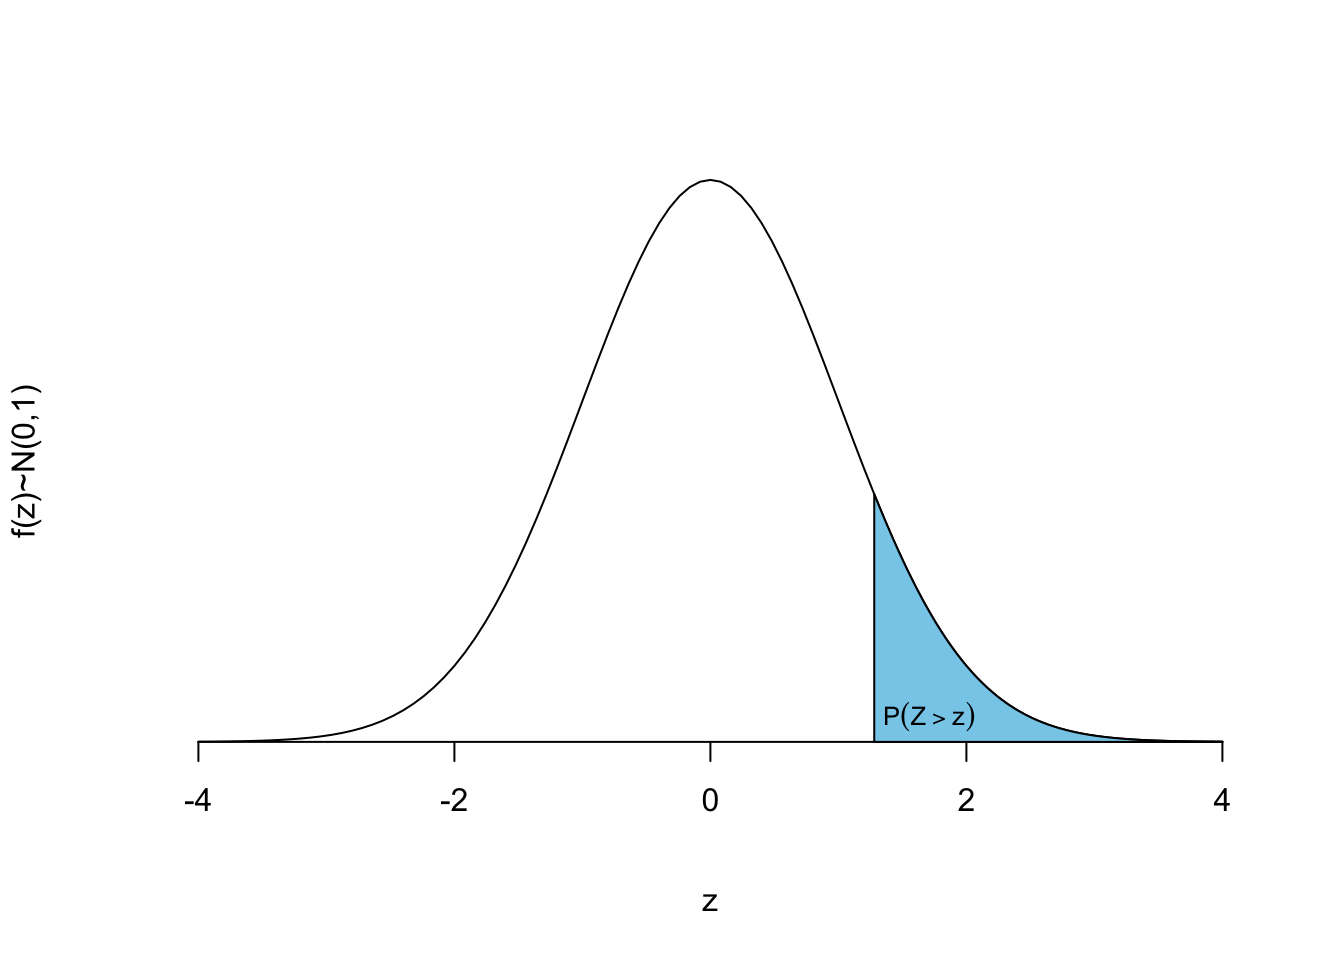
\includegraphics[width=0.7\linewidth]{91-apendices_files/figure-latex/unnamed-chunk-2-1}

\begin{tabular}{r|r|r|r|r|r|r|r|r|r|r}
\hline
z & 0.00 & 0.01 & 0.02 & 0.03 & 0.04 & 0.05 & 0.06 & 0.07 & 0.08 & 0.09\\
\hline
0.0 & 0.5000 & 0.4960 & 0.4920 & 0.4880 & 0.4840 & 0.4801 & 0.4761 & 0.4721 & 0.4681 & 0.4641\\
\hline
0.1 & 0.4602 & 0.4562 & 0.4522 & 0.4483 & 0.4443 & 0.4404 & 0.4364 & 0.4325 & 0.4286 & 0.4247\\
\hline
0.2 & 0.4207 & 0.4168 & 0.4129 & 0.4090 & 0.4052 & 0.4013 & 0.3974 & 0.3936 & 0.3897 & 0.3859\\
\hline
0.3 & 0.3821 & 0.3783 & 0.3745 & 0.3707 & 0.3669 & 0.3632 & 0.3594 & 0.3557 & 0.3520 & 0.3483\\
\hline
0.4 & 0.3446 & 0.3409 & 0.3372 & 0.3336 & 0.3300 & 0.3264 & 0.3228 & 0.3192 & 0.3156 & 0.3121\\
\hline
0.5 & 0.3085 & 0.3050 & 0.3015 & 0.2981 & 0.2946 & 0.2912 & 0.2877 & 0.2843 & 0.2810 & 0.2776\\
\hline
0.6 & 0.2743 & 0.2709 & 0.2676 & 0.2643 & 0.2611 & 0.2578 & 0.2546 & 0.2514 & 0.2483 & 0.2451\\
\hline
0.7 & 0.2420 & 0.2389 & 0.2358 & 0.2327 & 0.2296 & 0.2266 & 0.2236 & 0.2206 & 0.2177 & 0.2148\\
\hline
0.8 & 0.2119 & 0.2090 & 0.2061 & 0.2033 & 0.2005 & 0.1977 & 0.1949 & 0.1922 & 0.1894 & 0.1867\\
\hline
0.9 & 0.1841 & 0.1814 & 0.1788 & 0.1762 & 0.1736 & 0.1711 & 0.1685 & 0.1660 & 0.1635 & 0.1611\\
\hline
1.0 & 0.1587 & 0.1562 & 0.1539 & 0.1515 & 0.1492 & 0.1469 & 0.1446 & 0.1423 & 0.1401 & 0.1379\\
\hline
1.1 & 0.1357 & 0.1335 & 0.1314 & 0.1292 & 0.1271 & 0.1251 & 0.1230 & 0.1210 & 0.1190 & 0.1170\\
\hline
1.2 & 0.1151 & 0.1131 & 0.1112 & 0.1093 & 0.1075 & 0.1056 & 0.1038 & 0.1020 & 0.1003 & 0.0985\\
\hline
1.3 & 0.0968 & 0.0951 & 0.0934 & 0.0918 & 0.0901 & 0.0885 & 0.0869 & 0.0853 & 0.0838 & 0.0823\\
\hline
1.4 & 0.0808 & 0.0793 & 0.0778 & 0.0764 & 0.0749 & 0.0735 & 0.0721 & 0.0708 & 0.0694 & 0.0681\\
\hline
1.5 & 0.0668 & 0.0655 & 0.0643 & 0.0630 & 0.0618 & 0.0606 & 0.0594 & 0.0582 & 0.0571 & 0.0559\\
\hline
1.6 & 0.0548 & 0.0537 & 0.0526 & 0.0516 & 0.0505 & 0.0495 & 0.0485 & 0.0475 & 0.0465 & 0.0455\\
\hline
1.7 & 0.0446 & 0.0436 & 0.0427 & 0.0418 & 0.0409 & 0.0401 & 0.0392 & 0.0384 & 0.0375 & 0.0367\\
\hline
1.8 & 0.0359 & 0.0351 & 0.0344 & 0.0336 & 0.0329 & 0.0322 & 0.0314 & 0.0307 & 0.0301 & 0.0294\\
\hline
1.9 & 0.0287 & 0.0281 & 0.0274 & 0.0268 & 0.0262 & 0.0256 & 0.0250 & 0.0244 & 0.0239 & 0.0233\\
\hline
2.0 & 0.0228 & 0.0222 & 0.0217 & 0.0212 & 0.0207 & 0.0202 & 0.0197 & 0.0192 & 0.0188 & 0.0183\\
\hline
2.1 & 0.0179 & 0.0174 & 0.0170 & 0.0166 & 0.0162 & 0.0158 & 0.0154 & 0.0150 & 0.0146 & 0.0143\\
\hline
2.2 & 0.0139 & 0.0136 & 0.0132 & 0.0129 & 0.0125 & 0.0122 & 0.0119 & 0.0116 & 0.0113 & 0.0110\\
\hline
2.3 & 0.0107 & 0.0104 & 0.0102 & 0.0099 & 0.0096 & 0.0094 & 0.0091 & 0.0089 & 0.0087 & 0.0084\\
\hline
2.4 & 0.0082 & 0.0080 & 0.0078 & 0.0075 & 0.0073 & 0.0071 & 0.0069 & 0.0068 & 0.0066 & 0.0064\\
\hline
2.5 & 0.0062 & 0.0060 & 0.0059 & 0.0057 & 0.0055 & 0.0054 & 0.0052 & 0.0051 & 0.0049 & 0.0048\\
\hline
2.6 & 0.0047 & 0.0045 & 0.0044 & 0.0043 & 0.0041 & 0.0040 & 0.0039 & 0.0038 & 0.0037 & 0.0036\\
\hline
2.7 & 0.0035 & 0.0034 & 0.0033 & 0.0032 & 0.0031 & 0.0030 & 0.0029 & 0.0028 & 0.0027 & 0.0026\\
\hline
2.8 & 0.0026 & 0.0025 & 0.0024 & 0.0023 & 0.0023 & 0.0022 & 0.0021 & 0.0021 & 0.0020 & 0.0019\\
\hline
2.9 & 0.0019 & 0.0018 & 0.0018 & 0.0017 & 0.0016 & 0.0016 & 0.0015 & 0.0015 & 0.0014 & 0.0014\\
\hline
3.0 & 0.0013 & 0.0013 & 0.0013 & 0.0012 & 0.0012 & 0.0011 & 0.0011 & 0.0011 & 0.0010 & 0.0010\\
\hline
3.1 & 0.0010 & 0.0009 & 0.0009 & 0.0009 & 0.0008 & 0.0008 & 0.0008 & 0.0008 & 0.0007 & 0.0007\\
\hline
3.2 & 0.0007 & 0.0007 & 0.0006 & 0.0006 & 0.0006 & 0.0006 & 0.0006 & 0.0005 & 0.0005 & 0.0005\\
\hline
3.3 & 0.0005 & 0.0005 & 0.0005 & 0.0004 & 0.0004 & 0.0004 & 0.0004 & 0.0004 & 0.0004 & 0.0003\\
\hline
3.4 & 0.0003 & 0.0003 & 0.0003 & 0.0003 & 0.0003 & 0.0003 & 0.0003 & 0.0003 & 0.0003 & 0.0002\\
\hline
3.5 & 0.0002 & 0.0002 & 0.0002 & 0.0002 & 0.0002 & 0.0002 & 0.0002 & 0.0002 & 0.0002 & 0.0002\\
\hline
3.6 & 0.0002 & 0.0002 & 0.0001 & 0.0001 & 0.0001 & 0.0001 & 0.0001 & 0.0001 & 0.0001 & 0.0001\\
\hline
3.7 & 0.0001 & 0.0001 & 0.0001 & 0.0001 & 0.0001 & 0.0001 & 0.0001 & 0.0001 & 0.0001 & 0.0001\\
\hline
3.8 & 0.0001 & 0.0001 & 0.0001 & 0.0001 & 0.0001 & 0.0001 & 0.0001 & 0.0001 & 0.0001 & 0.0001\\
\hline
3.9 & 0.0000 & 0.0000 & 0.0000 & 0.0000 & 0.0000 & 0.0000 & 0.0000 & 0.0000 & 0.0000 & 0.0000\\
\hline
\end{tabular}

\hypertarget{resumen-modelos-de-distribuciuxf3n-de-probabilidad}{%
\section{Resumen modelos de distribución de probabilidad}\label{resumen-modelos-de-distribuciuxf3n-de-probabilidad}}

\begin{tabular}{l|l|l|l}
\hline
Distribución & Probabilidad/Densidad/Distribución & Esperanza & Varianza\\
\hline
\$\textbackslash{}text\{Bernoulli\}\textbackslash{}\textbackslash{} \textbackslash{}mathit\{Ber\}(p)\$ & \$X = \textbackslash{}begin\{cases\} 1 \& \textbackslash{}mbox\{ con probabilidad \} p \textbackslash{}\textbackslash{} 0 \& \textbackslash{}mbox\{ con probabilidad \} 1-p \textbackslash{}end\{cases\}\$ & \$p\$ & \$p(1-p)\$\\
\hline
\end{tabular}

\hypertarget{repaso}{%
\chapter{Repaso}\label{repaso}}

\hypertarget{logaritmos-y-exponenciales}{%
\section{Logaritmos y exponenciales}\label{logaritmos-y-exponenciales}}

\hypertarget{ap:combinatoria}{%
\section{Combinatoria}\label{ap:combinatoria}}

Una de las definiciones de probabilidad implica \textbf{contar}
el número de veces que puede ocurrir un suceso determinado. Por tanto,
en muchas ocasiones el cálculo de probabilidades empieza contando las
posibilidades de que ocurra un suceso. La Combinatoria es la parte de la
Matemática discreta que nos ayuda en esta tarea. Incluimos un breve
resumen con ejemplos de las fórmulas más habituales y su cálculo con R.

\hypertarget{ejemplo-ilustrativo}{%
\subsection{Ejemplo ilustrativo}\label{ejemplo-ilustrativo}}

Habitualmente se utilizan ejemplos de juegos de azar para introducir el
cálculo de probabilidades, como lanzamiendo de monedas y dados, o
combinaciones de cartas en barajas de naipes. Para darle un enfoque
práctico, utilizaremos a lo largo del módulo un ejemplo ilustrativo que,
aunque totalmente inventado, se puede encontrar el lector
en el futuro con ligeras variaciones según su ámbito de actuación.
Utilizaremos en lo posible las cifras usadas en los problemas de azar
para ver la utilidad de aquéllos ejemplos en casos más prácticos.

Datos básicos:

\begin{itemize}
\item
  52 posibles usuarios de un servicio
\item
  La mitad son mujeres
\item
  4 directivos, 12 mandos, resto operarios
\item
  13 jóvenes, 26 adultos, 13 mayores (5, 18 y 3 mujeres en cada
  grupo respectivamente)
\item
  1 de cada seis hombres contratará el servicio (el doble si es mujer)
\end{itemize}

Nótese cómo podemos \emph{traducir} el concepto de
servicio a cualquier ámbito: usuarios de salud o educación, enfermos de
una determinada patología, equipos de una infraestructura, etc. Asimismo
las categorías pueden ser cualesquiera aplicables a los elementos de los
conjuntos.

\hypertarget{principio-buxe1sico-de-conteo}{%
\subsection{Principio básico de conteo}\label{principio-buxe1sico-de-conteo}}

\textbf{Definición}: Realizamos \(k\) experimentos sucesivamente, cada
uno de ellos con \(n_i\) posibles resultados (\(i=1, \ldots, k\)). Entonces
el número total de resultados posibles es:

\[n_1\cdot n_2, \cdot \ldots \cdot n_k\]

\textbf{Ejemplo}: Resultados posibles si tomamos al azar un individuo
y observamos su grupo de edad y si contratará o no el servicio.

\textbf{Código}

\begin{Shaded}
\begin{Highlighting}[]
\DecValTok{3}\SpecialCharTok{*}\DecValTok{2}
\CommentTok{\#\textgreater{} [1] 6}
\end{Highlighting}
\end{Shaded}

\hypertarget{permutaciones}{%
\subsection{Permutaciones}\label{permutaciones}}

\textbf{Definición}: De cuántas formas posibles podemos ordenar un
conjunto de \(n\) elementos sin repetirlos.

\[P_n = n! = n\cdot(n-1)\cdot(n-2)\cdot\ldots\cdot 2\cdot 1\]

\textbf{Ejemplo}: De cuántas formas podemos ordenar un conjunto de
tres individuos, uno de cada categoría laboral.

\textbf{Código}

\begin{Shaded}
\begin{Highlighting}[]
\FunctionTok{factorial}\NormalTok{(}\DecValTok{3}\NormalTok{)}
\CommentTok{\#\textgreater{} [1] 6}
\end{Highlighting}
\end{Shaded}

\hypertarget{variaciones-muestreo-sin-reemplazamiento}{%
\subsection{Variaciones (muestreo sin reemplazamiento)}\label{variaciones-muestreo-sin-reemplazamiento}}

\textbf{Definición}: De cuántas formas posibles podemos seleccionar
una muestra de \(n\) elementos de un conjunto total de \(m\), sin que se
repitan. Una ordenación distinta, es una posibilidad distinta.

\[V_{m,n} = m\cdot(m-1)\cdot(m-2)\cdot\ldots\cdot (m-n+1) = \frac{m!}{(m-n)!}\]

\textbf{Ejemplo}: De cuántas formas podemos seleccionar una muestra
de 5 individuos en nuestro conjunto de 52 sin que se repitan (por
ejemplo para asignar un ranking)

\textbf{Código}

\begin{Shaded}
\begin{Highlighting}[]
\FunctionTok{factorial}\NormalTok{(}\DecValTok{52}\NormalTok{)}\SpecialCharTok{/}\FunctionTok{factorial}\NormalTok{(}\DecValTok{52{-}5}\NormalTok{)}
\CommentTok{\#\textgreater{} [1] 311875200}
\end{Highlighting}
\end{Shaded}

\hypertarget{variaciones-con-repeticiuxf3n-muestreo-con-reemplazamiento}{%
\subsection{Variaciones con repetición (muestreo con reemplazamiento)}\label{variaciones-con-repeticiuxf3n-muestreo-con-reemplazamiento}}

\textbf{Definición}: De cuántas formas posibles podemos seleccionar
una muestra de \(n\) elementos de un conjunto total de \(m\), pudiéndose
repetir. Una ordenación distinta, es una posibilidad distinta.
\[\mathit{VR}_{m,n} = m^n\]

\textbf{Ejemplo}: De cuántas formas podemos seleccionar una muestra
de 5 individuos en nuestro conjunto de 52 pudiéndose repetir (por
ejemplo para asignar premios consecutivamente)

\textbf{Código}

\begin{Shaded}
\begin{Highlighting}[]
\DecValTok{52}\SpecialCharTok{\^{}}\DecValTok{5}
\CommentTok{\#\textgreater{} [1] 380204032}
\end{Highlighting}
\end{Shaded}

\hypertarget{combinaciones-muestras-equivalentes}{%
\subsection{Combinaciones (muestras equivalentes)}\label{combinaciones-muestras-equivalentes}}

\textbf{Definición}: De cuántas formas posibles podemos seleccionar
una muestra de \(n\) elementos de un conjunto total de \(m\), sin importar
el orden.

\[\mathit{C}_{m,n} = \binom{m}{n} = \frac{m!}{n!(m-n)!}\]

\(\binom{m}{n}\) se lee \emph{m sobre n}, y se le conoce como \emph{número combinatorio}.
Algunas propiedades importantes de los números combinatorios:

\[\binom{m}{m} = \binom{m}{0} = 1.\]
\[\binom{m}{1} = \binom{m}{m-1} = m.\]
\[\binom{m}{n} + \binom{m}{n+1} = \binom{m+1}{n+1}\]
Por otra parte, por convenio se tiene que:

\[0!=1,\]

\[\text{si } a <b \implies \binom{a}{b} = 0.\]

\textbf{Ejemplo}: De cuántas formas podemos seleccionar una muestra
de 5 individuos en nuestro conjunto de 52 sin importar el orden (por
ejemplo para asignar premios de una sola vez)

\textbf{Código}

\begin{Shaded}
\begin{Highlighting}[]
\FunctionTok{choose}\NormalTok{(}\DecValTok{52}\NormalTok{, }\DecValTok{5}\NormalTok{)}
\CommentTok{\#\textgreater{} [1] 2598960}
\end{Highlighting}
\end{Shaded}

\hypertarget{combinaciones-y-permutaciones-con-repeticiuxf3n}{%
\subsection{Combinaciones y permutaciones con repetición}\label{combinaciones-y-permutaciones-con-repeticiuxf3n}}

Las combinaciones y
permutaciones también se pueden dar con repetición, siendo las fórmulas
para calcularlas las siguientes:

\[\mathit{CR}_{m,n}= \mathit{C}_{m+n-1,n}= \frac{(m+n-1)!}{n!\cdot(m-1)!}\]
\[\mathit{PR} = \frac{n!}{a!\cdot b!\cdot \ldots\cdot z!}\]

La primera situación es aquella en la que los
elementos se pueden repetir, pero no nos importa el orden en que lo
hagan. La segunda aparece cuando el elemento A del conjunto total de
elementos aparece \(a\) veces, y así sucesivamente.

\hypertarget{ampliaciuxf3n}{%
\chapter{Ampliación}\label{ampliaciuxf3n}}

En este apéndice se incluyen temas avanzados que pueden ser útiles al lector
más allá de un curso básico de estadística económica y empresarial, y
que no se han incluido en el cuerpo de los capítulos para mantener el nivel
de un primer curso de grado.

\hypertarget{funciuxf3n-caracteruxedstica}{%
\section{Función característica}\label{funciuxf3n-caracteruxedstica}}

\hypertarget{cambio-de-variable}{%
\section{Cambio de variable}\label{cambio-de-variable}}

\hypertarget{variables-aleatorias-unidimensionales-mixtas}{%
\section{Variables aleatorias unidimensionales mixtas}\label{variables-aleatorias-unidimensionales-mixtas}}

\hypertarget{variables-aleatorias-bidimensionales-mixtas}{%
\section{Variables aleatorias bidimensionales mixtas}\label{variables-aleatorias-bidimensionales-mixtas}}

\hypertarget{algunos-modelos-de-distribuciuxf3n-continuos-muxe1s}{%
\section{Algunos modelos de distribución continuos más}\label{algunos-modelos-de-distribuciuxf3n-continuos-muxe1s}}

\hypertarget{modelos-de-distribuciuxf3n-de-probabilidad-multivariantes}{%
\section{Modelos de distribución de probabilidad multivariantes}\label{modelos-de-distribuciuxf3n-de-probabilidad-multivariantes}}

\hypertarget{modelos-de-distribuciuxf3n-de-probabilidad-relacionadas-con-la-normal}{%
\section{Modelos de distribución de probabilidad relacionadas con la normal}\label{modelos-de-distribuciuxf3n-de-probabilidad-relacionadas-con-la-normal}}

\hypertarget{simulaciuxf3n-de-variables-aleatorias}{%
\section{Simulación de variables aleatorias}\label{simulaciuxf3n-de-variables-aleatorias}}

\(U(0;\; 1)\): Generador de probabilidades aleatorias. Dada cualquier función de distribución \(F\), se pueden generar valores de esa VA obteniendo \(F^{-1}(U(0;\; 1))\)

\hypertarget{demostraciones}{%
\chapter{Demostraciones}\label{demostraciones}}

Em este apéndice se incluyen aquellas demostraciones de teoremas y propiedades
no incluidas en los capítulos para mantener el carácter práctico del mismo.

\hypertarget{variable-aleatoria-discreta}{%
\section{Variable aleatoria discreta}\label{variable-aleatoria-discreta}}

\hypertarget{funciuxf3n-de-probabilidad}{%
\subsection{Función de probabilidad}\label{funciuxf3n-de-probabilidad}}

\hypertarget{esperanza}{%
\subsection{Esperanza}\label{esperanza}}

\hypertarget{varianza}{%
\subsection{Varianza}\label{varianza}}

\hypertarget{creditos}{%
\chapter{Créditos}\label{creditos}}

Los gráficos y diagramas generados son creación y propiedad del autor, salvo que se
indique lo contrario. Su licencia de uso es la misma que la del resto de la
obra, véase el Prefacio.

\begin{itemize}
\item
  Las imágenes de tipo \emph{clipart} usadas en esta obra y las fotografías no atribuidas
  pertenecen al dominio público gracias a \href{http://www.openclipart.org}{openclipart.org}, \href{https://unsplash.com}{unplash.com} o \href{https://pixabay.com/es/}{pixabay.com}.
\item
  The \href{https://www.r-project.org/logo/}{R logo} is (c) 2016 The R Foundation.
\end{itemize}

  \bibliography{book.bib,packages.bib}

\end{document}
